%% $Id: louveaux-epfl06.tex,v 1.5 2006/07/10 13:46:20 louveaux Exp $
%%\documentclass[9pt,trans]{beamer}
\documentclass[9pt]{beamer}
\usepackage{beamerfoils}%% FoilTeX emulation
\usepackage{epsfig}
\usepackage{eurosym}
\mode<presentation>
{
  \usetheme{Boadilla}
  % oder ...

  \setbeamercovered{transparent}
  % oder auch nicht
}
\usepackage[french]{babel}
\usepackage[latin1]{inputenc}
%%\usepackage{times}
%%\usepackage[T1]{fontenc}
%\usepackage{booktabs}

%%\includeonlyframes{current}

\title{Discrete Optimization}

\author{Quentin
Louveaux}
\institute{ULg - Institut Montefiore}
\date{2016}

% Falls eine Logodatei namens "university-logo-filename.xxx" vorhanden
% ist, wobei xxx ein von latex bzw. pdflatex lesbares Graphikformat
% ist, so kann man wie folgt ein Logo einf|gen:

% \pgfdeclareimage[height=0.5cm]{university-logo}{university-logo-filename}
% \logo{\pgfuseimage{university-logo}}

% Folgendes sollte gelvscht werden, wenn man nicht am Anfang jedes
% Unterabschnitts die Gliederung nochmal sehen mvchte.
%% \AtBeginSection[]
%% {
%%   \begin{frame}<beamer>
%%     \frametitle{Gliederung}
%%     \tableofcontents[currentsection,currentsubsection]
%%   \end{frame}
%% }

% Falls Aufzdhlungen immer schrittweise gezeigt werden sollen, kann
% folgendes Kommando benutzt werden:

\beamerdefaultoverlayspecification{<+->}

%%%%%%
\definecolor{rot}{rgb}{1,0,0}
\definecolor{gruen}{rgb}{0,1,0}
\definecolor{blau}{rgb}{0,0,1}

%%% number sets
\newcommand{\Z}       {\mathbb{Z} }
\newcommand{\R}       {\mathbb{R} }
\newcommand{\Q}       {\mathbb{Q} }
\newcommand{\N}       {\mathbb{N} }
\newcommand{\spa}     {\text{span}}
\newcommand{\lin}     {\text{span}}
\newcommand{\inter}   {\text{int} }


%%% mathematical stuff
\newcommand{\sosR}    {\sum^2}
\newcommand*{\transpose}[1]  { {#1}^T }
\newcommand*{\rounddown}[1]  {\left\floor #1 \right\rfloor}
\newcommand*{\roundup}[1]    {\left\lceil  #1 \right\rceil}
\newcommand*{\ipart}[1]      {\rounddown{#1}}
\newcommand*{\fpart}[1]      {\mathfrak{f}\left(#1\right)}


\newcommand*{\iepoly}[2]  {z_{#1}\left(#2\right)}
\newcommand*{\redmon}[3]  {r_{#1}^{#2}\left( #3 \right)}
\newcommand*{\redset}[1]  {#1^{\emph{red}}}

\newcommand*{\Gpoly}[1] {P_{[#1]}}

\newcommand*{\nonc}[1]{\overline{#1}}
\newcommand*{\const}[1]{#1_0}

\newcommand{\define}{\stackrel{\rm def.}{\Leftrightarrow}}
\newcommand{\qform}[3]{\frac{1}{2} x^{\top}#1x + #2^{\top}x + #3}
\def\xzero{x^{0}}
\newcommand{\gxh}[2]{{g_{#1}(#2)}}

\def\pcone_k{{\mathcal C}_{k}(f)}
\def\orthant_j{{\mathcal O}_{j}}

\def\BDB{BDB^{\top}}
\def\LDL{LDL^{\top}}
\def\bA{A}
\def\bb{b}
\def\bc{c}
\def\bh{h}
\def\bp{p}
\def\bx{x}
\def\by{y}
\def\bu{u}
\def\bv{v}
\def\bd{d}
\def\T{^{T}}
\def\D{}
\def\mb{{\bf}}
\def\sep{}
\def\bo{0}
\def\bw{w}
\def\ba{a}
\def\bg{g}
\def\bH{H}
\def\be{e}

\let\ve=\relax
\newcommand\vealpha{{\alpha}}
\newcommand{\st}{\mathrm{s.t.}}
\DeclareMathOperator\conv{conv}
\DeclareMathOperator\cone{cone}
\newcommand{\B}{\{0,1\}}

\newcommand*{\person}[1] {\textsc{#1}}

\newtheorem{algorithm}{Algorithmus}

\makeatletter
\newenvironment{rmat}{\left(\null\,\vcenter\bgroup
  \Let@\restore@math@cr\default@tag
  \baselineskip6\ex@ \lineskip1.5\ex@ \lineskiplimit\lineskip
  \ialign\bgroup\hfil$\m@th\scriptstyle##$&&\thickspace
  \hfil$\m@th\scriptstyle##$\crcr
}{%
  \crcr\egroup\egroup\,\right)%
}
\makeatother

%%%%%%%%%%%%%%%%%%%%%%%%%%%%%%%%%%%%%%%%%%%%%%%%%%%%%%%%%%%%%%%%%%%%%%%%%%%%%%%%
%\begin{frame}
  %\titlepage
%\end{frame}

%% \begin{frame}
%%   \frametitle{Gliederung}
%%   \tableofcontents
%%   % Die Option [pausesections] kvnnte n|tzlich sein.
%% \end{frame}


%%%%%%%%%%%%%%%%%%%%%%%%%%%%%%%%%%%%%%%%%%%%%%%%%%%%%%%%%%%%%%%%%%

\definecolor{orange}{rgb}{0.8,0.3,0.0}
\definecolor{darkgreen}{rgb}{0.0,0.5,0.0}
\definecolor{gold}{rgb}{1.0,0.8,0.0}
\definecolor{brown}{rgb}{0.6,0.2,0.2}
\definecolor{blue4}{rgb}{0,0,144}
\definecolor{white}{rgb}{255,255,255}
\definecolor{blueexample}{rgb}{0.2,0.2,0.7}
\begin{document}
\begin{frame}
  \titlepage
\end{frame}
\begin{frame}
\frametitle{Dealing with a (NP-)hard problem}
\begin{block}{Bounding the solution}
\begin{itemize}
\item<1-> Need of a \alert{primal bound} (upper bound in the case of a minimization problem)\medskip
\item<1-> Need of a \alert{dual bound} (lower bound in the case of a minimization problem)\medskip
\end{itemize}
When the two bounds \alert{meet}, we have a proof of \alert{optimality}.
\end{block}
\end{frame}
\begin{frame}
\frametitle{The primal bound}
A \alert{primal bound} is a \alert{lower bound} to the value of the optimal solution for a maximization.\medskip

A \alert{primal bound} is an \alert{upper bound} to the value ofthe  optimal solution for a minimization.\bigskip

How to find a primal bound?\bigskip

By finding a \alert{feasible solution} to the problem.\\
The best possible primal bound is given by the \alert{optimal solution}.
\end{frame}
\begin{frame}
\frametitle{The dual bound}
A \alert{dual bound} is an \alert{upper bound} to the value of the  optimal solution for a maximization.\medskip
A \alert{dual bound} is a \alert{lower bound} to the value of the  optimal solution for a minimization.\bigskip

How to find a dual bound?\bigskip

There are several ways.\\
We will cover two ways: through \alert{relaxations}, through \alert{Lagrangian duality}.
\end{frame}
\begin{frame}
\frametitle{Relaxations}
Consider an optimization problem:
\begin{align*}
\min \; & c(x)\\
\text{s.t. } 
& x\in X.
\end{align*}
A \alert{relaxation} is an (easier) optimization problem for which the value of the optimal solution
is \alert{guaranteed to be lower} than that of the initial problem.
\begin{block}{Ways to obtain a relaxation}
\begin{itemize}
\item<1-> Enlarge the \alert{feasible set} $Y\supseteq X$ and solve
\begin{align*}
\min \; & c(x)\\
\text{s.t. } 
& x\in \alert{Y}.
\end{align*}
\item<1-> Replace the \alert{objective function} $c(x)$ by a \alert{lower value} $d(x)$ for every feasible $x$,
i.e. $d(x)\leq c(x) $ for all $x\in X.$
\begin{align*}
\min \; & d(x)\\
\text{s.t. } 
& x\in X.
\end{align*}
\item<1-> Or \alert{combine} the two.
\end{itemize}
Note: if we replace the feasible set by a  \alert{smaller set} $Y\subseteq X$, we talk about a \alert{restriction} which may be useful
to find \alert{primal bounds}.
\end{block}
\end{frame}
\begin{frame}
\frametitle{The linear programming relaxation}
For a mixed-integer optimization problem  of the form
\begin{align*}
\min \; & c^Tx+d^Ty\\
\text{s.t. } 
& Ax+Gy\leq b\\
&x\in \mathbb Z^n_+, y\in \mathbb R^m_+,
\end{align*}
the \alert{linear programming relaxation} consists in replacing the \alert{integrality constraints}
by simple \alert{nonnegativity constraints}:
\begin{align*}
\min \; & c^Tx+d^Ty\\
\text{s.t. } 
& Ax+Gy\leq b\\
&x\in \alert{\mathbb R^n_+}, y\in \mathbb R^m_+.
\end{align*}
The set of \alert{feasible solutions} is now larger than before.
\end{frame}
\begin{frame}
\frametitle{The linear programming relaxation}
For a mixed-integer optimization problem  of the form
\begin{align*}
\min \; & c^Tx+d^Ty\\
\text{s.t. } 
& Ax+Gy\leq b\\
&x\in \{0,1\}^n, y\in \mathbb R^m_+,
\end{align*}
the \alert{linear programming relaxation} consists in replacing the \alert{integrality constraints}
by simple \alert{nonnegativity constraints}:
\begin{align*}
\min \; & c^Tx+d^Ty\\
\text{s.t. } 
& Ax+Gy\leq b\\
&x\in \alert{[0,1]}, y\in \mathbb R^m_+.
\end{align*}
The set of \alert{feasible solutions} is now larger than before.
\end{frame}
\begin{frame}
\frametitle{When the linear programming relaxation tells you everything}
Two lucky cases allow us to solve a problem just with the linear programming relaxation.
\begin{block}{Proposition}
\begin{itemize}
\item<1-> If the linear programming relaxation of a mixed-integer optimization problem is \alert{infeasible},
then the mixed-integer optimization problem is \alert{infeasible} as well.\bigskip
\item<1-> If an optimal solution of the linear programming relaxation of a mixed-integer optimization problem is
\alert{integral} then it is also \alert{optimal } for the mixed-integer optimization problem.
\end{itemize}
\end{block}
\end{frame}
\begin{frame}
\frametitle{Branch-and-Bound}
Idea: enumerate but \alert{using the information} of the linear relaxation.
\begin{overlayarea}{\linewidth}{5cm}
\begin{center}
\includegraphics<2>[height=5cm]{bb0.pdf}
\includegraphics<3-4>[height=5cm]{bb1.pdf}
\includegraphics<5-6>[height=5cm]{bb2.pdf}
\end{center}
\end{overlayarea}
\uncover<2->{LP Solution: $x^{1*} = (\frac{265}{79},\frac{160}{79})$
with optimal cost $12.79$}
\begin{overlayarea}{\linewidth}{1.2cm}
\only<3-4>{2 branches are created: either $x_1\geq 4$ or $x_1\leq 3$\\
Branch 1: $x_1\geq 4$ : $x^{2*}=(4,\frac{1}{4})$ with optimal cost $8.75$\\
\alert{Prune by bound} if we suppose $x=(0,3)$ with cost 9 is known.\\}
\only<5-6>{2 further branches are created: either $x_2\leq 2$ or $x_2\geq 3$\\
Branch 2.1: $x_2\leq 2$ : $x^{4*}=(3,2)$ with optimal cost $12$\\
\alert{Prune by optimality} \\}
\end{overlayarea}
\begin{overlayarea}{\linewidth}{1cm}
\only<4>{Branch 2: $x_1\leq 3$ : $x^{3*} = (3,\frac{20}{9})$ with optimal cost $12.67$}
\only<6>{Branch 2.2: $x_2\geq 3$ : $x^{5*} = (\frac{8}{5},3)$ with optimal cost $12.2$\\
2 further branches: $x_1\leq 1$ which gives $(1,3)$ (prune by optimality and bound)
and $x_1\geq 2$ (\alert{prune by infeasiblity})}
\end{overlayarea}
\end{frame}
\begin{frame}
\frametitle{Summary of the branch-and-bound tree}
\begin{center}
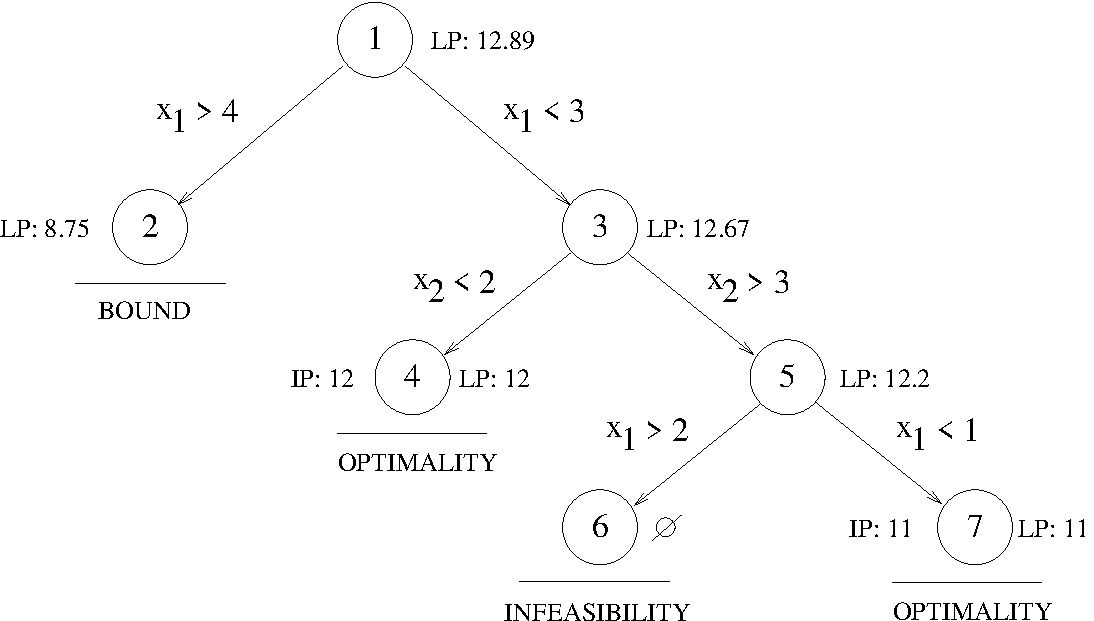
\includegraphics[height=7cm]{bbtree.pdf}
\end{center}
\end{frame}
\begin{frame}
\frametitle{Branch-and-Bound}
\begin{block}{Remarks}
\begin{itemize}
\item<1-> Opportunities to prune the search:\\
\alert{By bound, By optimality, By infeasibility}
\item<1-> Need of a good \alert{primal bound} in the beginning
\item<1-> Different strategies for the \alert{node selection}:\\
depth-first-search (good to find quickly primal solutions)\\
breadth-first-search (good to increase the \alert{dual bound})\\
best node (optimal for the \alert{dual bound})
\item<1-> Different strategies for \alert{variable selection}:\\
Most fractional variable or least fractional variable\\
Look ahead for best improvement in the bound: \alert{strong branching}
Take advantage of the history of branching: \alert{reliability branching}\\
\end{itemize}
\end{block}
\end{frame}
\end{document}
